\section{An Extended Application: \\ Cryptographic Protocol Analysis}

	The chase can be used for protocol analysis. A common technique for the analysis
	of protocols involves identifying the \emph{essentially different} runs of
	the protocol. These essentially different protocol runs are analogous to
	minimal models. When a protocol is described using geometric logic, the
	chase can find such minimal models. The protocol can then be analysed for
	characteristics such as the existence of security violations or other
	unexpected behaviour.

	\subsection{Background}

		\subsubsection{Strand Spaces}

			The \emph{strand space formalism} was developed as a method for
			formally reasoning about cryptographic protocols. Participants in a
			protocol run are represented by \emph{strands}. The formalism
			distinguishes between two different kinds of participants: regular
			participants and an adversary. A regular participant is represented
			by a regular strand, and must follow the protocol. The adversary is
			represented by zero or more adversary strands, and can manipulate
			the messages that regular strands send/receive. A single physical
			entity can be represented as multiple regular strands if they play
			more than one role in the protocol.

			\paragraph{Messaging}

				A strand is made up of a non-empty, finite sequence of nodes.
				Every node either sends or receives a term, called its
				\emph{message}.  Terms are defined inductively as follows:

				\begin{itemize}
				\item any text is a term, specifically a \emph{basic term}
				\item the ciphertext $\{|\tau_1|\}_{\tau_2}$ is a term if the plaintext $\tau_1$ and the key $\tau_2$ are terms
				\item the pair ($\tau_1$,$\tau_2$) is a term if $\tau_1$ and $\tau_2$ are terms
				\end{itemize}

				A term $t$ is an \emph{ingredient} of another term $u$ if $u$
				can be constructed from $t$ by repeatedly pairing with
				arbitrary terms and encrypting with arbitrary keys.

				A \emph{nonce} is a uniquely-originating basic term. A term $t$
				\emph{originates} on a node $n$ of a strand $s$ if $n$ is a
				sending node, $t$ is an ingredient of the message of $n$, and
				$t$ is not an ingredient of any previous node on $s$. A term is
				\emph{uniquely originating} if it originates on only one
				strand. A term is non-originating if it does not appear in any
				strand.

				If a regular participant generates a random fresh nonce, it
				will be assumed uniquely-originating because of the extreme
				unlikelihood of any other participant generating and
				originating the same value.

				Similiarly, non-origination is helpful in describing private
				assymetric keys that should never be sent as part of a message.

			\paragraph{The Adversary}

				An adversary is included in the strand space formalism to
				represent a worst-case situation, where an attacker may control
				every point of communication between regular participants.  The
				actions of the advesary are represented by \emph{advesary
				strands}. Recall that adversary strands are not bound by the
				rules defined by the protocol; they manipulate messages being
				sent and received by non-adversarial strands.

				The capabilities of the adversary strands are given by the
				Dolev-Yao Threat Model \textbf{references}. The five possible
				operations that an adversary may perform are derived from both
				the Dolev-Yao Threat Model and the strand space formalism.
				These operations are:

				\begin{description}
				\item [pairing] the pairing of two terms
				\item [unpairing] the extraction of a term from a pair
				\item [encryption] given a key $k$ and a plaintext $m$, the construction of the ciphertext $\{|m|\}_k$ by encrypting $m$ with $k$
				\item [decryption] given a ciphertext $\{|m|\}_k$ and its decryption key $k^{-1}$, the extraction of the plaintext $m$
				\item [generation] the generation of an original term when that term is not assumed to be secure
				\end{description}

				Pairing and encryption are \emph{construction operations}.
				Decryption and unpairing are \emph{deconstruction operations}.

		\subsubsection{Cremers' Algorithm}

			\emph{Cremers' Algorithm} adds constraints to adversarial actions
			to allow one to infer the possible classes of protocol runs.

			Cremers gives two major constraints, which will be called
			``efficiency" and ``normalcy". A protocol is \emph{efficient} if an
			adversary always takes a message from the earliest point at which
			it appears. A protocol is \emph{normal} when the adversary is
			performing either a deconstruction or construction, it always
			performs zero or more deconstruction operations followed by zero or
			more construction operations, except in the case of constructing
			decryption keys. Cremers proved that these constraints do not limit
			the capabilities of an adversary \textbf{reference}.

			\textbf{above paragraph needs some rewriting}

			An important insight used in Cremers' algorithm, called
			\emph{chaining}, states that terms in messages received from an
			adversary strand always originate in a non-adversarial strand. In
			simpler terms, an adversary can not send a message to himself nor
			receive a message from himself.

	\subsection{The Problem}

		Some protocol researchers want to be able to programmatically reason
		about cryptographic protocols. A common technique for this is to find a
		set of essentially different classes of protocol runs, which are each a
		subset of all possible runs of the protocol. Together, these classes of
		protocol runs encompass every possible run of the protocol. This can be
		accomplished by finding minimal models of a geometric logic
		representation of the protocol. This happens to be precisely the
		problem the chase solves.

	\subsection{The Solution: Minimal Models}

		Given a theory $\mathcal{T}$, the jointly minimal models $\mathcal{M}$
		that the chase outputs are representative of all models because there
		always exists a homomorphism from some model $\mathbb{M} \in
		\mathcal{M}$ to any model that satisfies $\mathcal{T}$. Each model that
		satisfies $\mathcal{T}$ represents a class of runs of the protocol. The
		set of all models output by the chase represents every possible run of
		the protocol. Finding every possible run of the protocol is prohibitive
		because there are infinitely many. Because the set of models is
		countably infinite, they can be enumerated, but can not be listed.

	\subsection{Designing An Analogous Theory}

		In order to create a geometric theory describing a protocol, the
		formul{\ae} that define strand spaces, normilisation, efficiency, and
		chaining must be derived. The formul{\ae} defining the protocol must be
		combined with this scaffolding to create a theory that can be used to
		infer the possible runs of the protocol.

		The \emph{half-duplex protocol} was chosen to be used as an example.
		This protocol involves two participants, Alice and Bob. The protocol
		specifies that the following actions take place:

		\begin{enumerate}
		\item Alice sends Bob a nonce that she generated, encrypted with Bob's public key
		\item Bob receives the encrypted nonce
		\item Bob replies to Alice with the decrypted nonce
		\item Alice receives Bob's message
		\end{enumerate}

		This protocol can be visually represented as in Figure \ref{fig:half-duplex}.

		%\begin{figure}[h]
		%	\centering
		%	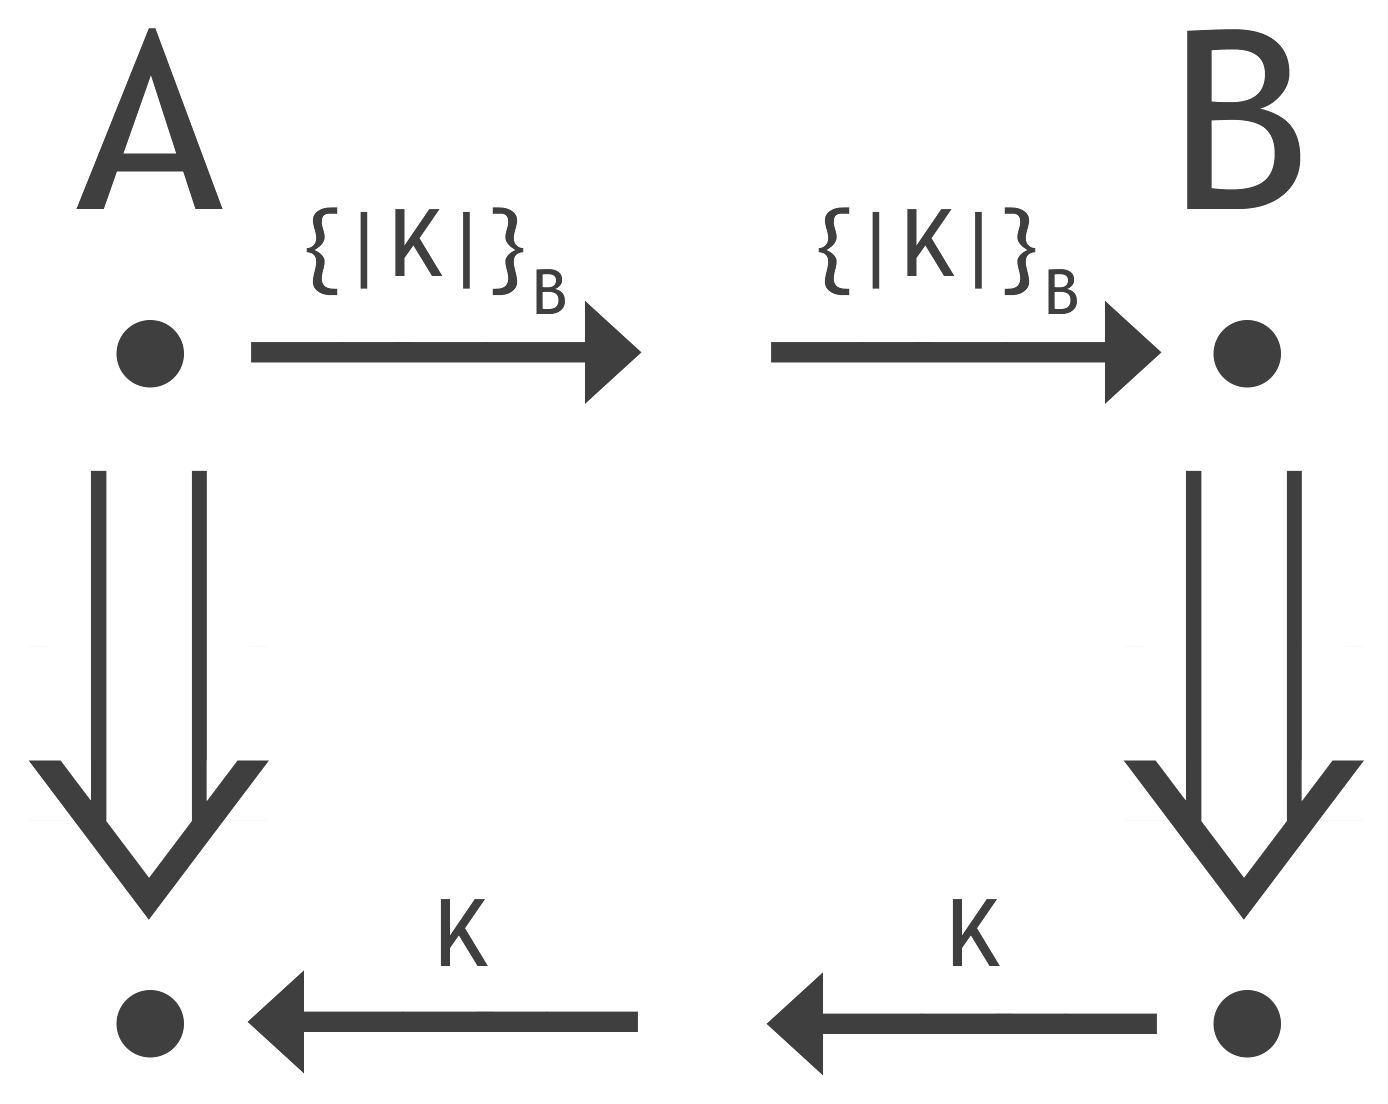
\includegraphics[width=0.6\textwidth]{half-duplex.png}
		%	\caption{
		%		A visual representation of the half-duplex protocol modeled in strand space
		%		\label{fig:half-duplex}
		%	}
		%\end{figure}

		The geometric logic rules that model this protocol were generated
		manually by direct translation into geometric logic. Ideally, the
		process of generating geometric logic formul{\ae} from protocols should
		be done automatically.

	\subsection{The Results}

		The chase was run on the logic representation of the half-duplex protocol.
		A single model was returned during the execution of the algorithm,
		which was manually stopped before natural completion. This model, like
		all models returned by the chase, satisfies the input theory, and
		belongs to a set of jointly minimal models for the theory. The returned
		model denotes a run of the protocol which contains no adversary strands
		and is a correct execution of the protocol.
